\section{Methodology}
\subsection{Problem formulation}
\label{sec:prob-formulation}
Given an input video containing $N$ frames, we want to produce a binary time series of same length $N$ such that each index $i$ predicts the labels $y_i$ of corresponding frame $f_i$ . Trespassing label is assigned to positive (1) class and non-trespassing label is assigned to negative class (0). Since, each prediction depends only on corresponding frame $f_i$, our problem boils down to determining a function $D$ such that 
$$ D(f_i) = \hat{y}_i $$
This function $D$ has parameters $\theta$ such that $D(f_i;\theta) = \hat{y}_i$. The aim is to find a $\theta^*$ such that $D(f_i;\theta) \rightarrow y_i$ where $y_i$ is the ground truth label corresponding to $f_i$. The ground truth label has the following definition: 
$$y=
\begin{cases}
1,  &\qquad \textrm{if } f_i \textrm{ has trespassing activity} \\ 
0, 	&\qquad \textrm{otherwise}
\end{cases}
$$
We define the trespassing activity as the presence of at  least one person in the frame. 
% Figure \ref{fig:trespassing-detection-block} shows a block diagram of problem. 




\subsection{Proposed pipeline} 
In order to tackle this problem, we propose a two-stage trespassing detection model. Figure \ref{fig:trespassing-detection-framework} shows the model framework. In the first stage, we decide whether a particular frame $f_i$ has activity or not. If it turns out that $f_i$ has no activity, then it is classified as background frame. This frame shall no longer be processed by second stage. On the other hand, if $f_i$ shows activity, then second stage shall investigate whether its human trespassing activity or not. Figure \ref{fig:trespassing-detection-pipeline} shows the block diagram of our system implementing trespassing detection framework. Stage 1 of our pipeline corresponds to level 1 of framework. Likewise, stage 2 of pipeline corresponds to level 2 of framework. Input to our pipeline is a video and each frame is processed one by one. Each frame is first processed through stage 1 to determine if it shows activity. Only the frames classified as showing activity are further processed through stage 2. Output of the system is a time series as discussed in section \ref{sec:prob-formulation}  

\begin{figure}
    \centering
    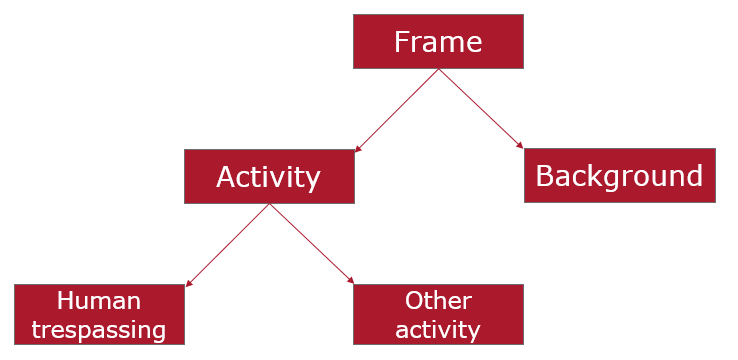
\includegraphics[width=\linewidth]{images/trespassing-detection-framework.PNG}
    \caption{Trespassing detection framework}
    \label{fig:trespassing-detection-framework}
\end{figure}

\begin{figure}
    \centering
    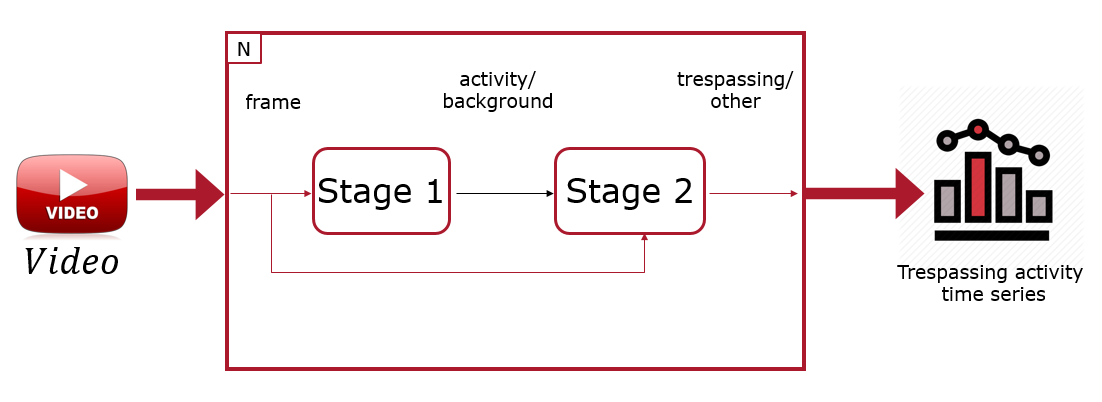
\includegraphics[width=\linewidth]{images/trespassing-detection-pipeline.PNG}
    \caption{Trespassing detection pipeline}
    \label{fig:trespassing-detection-pipeline}
\end{figure}

\subsection{Stage 1}
As discussed above, goal of this stage is to filter non-activity frames from the activity frames. Thus, it is modeled as a background subtraction problem. Figure \ref{fig:background-subtraction-model} shows a typical pipeline of background subtraction method. 

Input to this stage is the given frame $f_i$ in question. This frame $f_i$ is first used to update the background model from $b_{i-1}$ to $b_i$. Both $f_i$ and $b_i$ are then compared with each other by the foreground extraction sub-stage. Output of this sub-stage is a binary mask which indicates whether a pixel belongs to foreground or not. All the foreground pixels in the image can be summed up and their ratio to the the total no. of pixels in frame can be compared to a threshold value. If the ratio is greater than threshold, then it is a frame regarded as activity frame; otherwise it is classified as background frame. In this work, we use Mixture of Gaussian (MoG) and Google Summer of Code (GSoC) methods for background subtraction. We shall elaborate the working principal of MoG. 
\begin{figure}
    \centering
    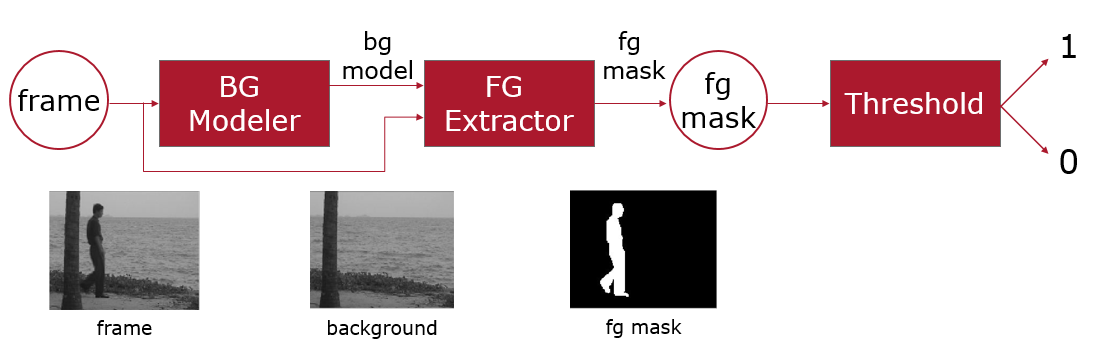
\includegraphics[width=\linewidth]{images/background-subtraction-model.PNG}
    \caption{Background subtraction model}
    \label{fig:background-subtraction-model}
\end{figure}

\subsubsection{Mixture of Gaussian (MoG)}
Before diving into the technical detail of MoG based background subtraction, let us explain it intuitively. This method attempts to model the pixel values as a gaussian process (normal distribution). Since, an image usually represents many different surfaces/objects, each surface/object is expected to give rise to a new gaussian. Thus all the pixel values are better represented by a mixture (sum) of gaussians. This is how gaussian mixture models an image. Notice that this model represents both foreground and background simultaneously. In order to apply this model to background subtraction problem, we associate each pixel with a particular surface and then associate that surface with either foreground or background. The label of each pixel (foreground/background) is determined by the label of corresponding surface. The methodology being described here is due to \cite{stauffer1999adaptive} and \cite{power2002understanding}

Each surface (or uniform object) that comes into the view is represented by a state $k \in {1,2,3,...,K}$. Some of these states correspond to  background while remaining ones are considered to be foreground. The process  $\mathbf{k}$ which generates the states is modeled by parameters set ${w_1, w_2, ..., w_K}$ where $w_k = P(k)$. Each of these parameters represents  a priori probability of surface $k$ appearing in the image. Further, $\sum_{k=1}^K w_k=1$. 

This surface process $\mathbf{k}$ is hidden and is only indirectly observable through pixel value process $X$. The pixel value process $\mathbf{X}$ is an observable random variable modeled by a gaussian process for given surface $k$. $\mathbf{X}$ is 1-D in case of gray scale images and 3-D for color images.  If $\theta_k= \{\mu_k, \Sigma_k \}$  represent the associated gaussian process then pixel value process $\mathbf{X}$ given $k$ is: 

$$ f_{\mathbf{X}|k}(X|k,\theta_k)=\frac{1}{\sqrt{(2\pi)^n |\Sigma_k |}}e^{-\frac{1}{2}(X-\mu_k)^T \Sigma_k^{-1} (X-\mu_k)} $$
where $\mu_k$ is the mean and $\Sigma_k$ is the covariance matrix of associated $k^{th}$ gaussian. 

We assume these $k$ events are disjoint so $\mathbf{X}$ can be modelled as sum of gaussians. 

$$ f_{\mathbf{X}}(X|\Phi)=\sum_{k=1}^K w_k f_{\mathbf{X}|k}(X|k,\theta_k)  $$
where $ \Phi = \{w_1, \mu_1, \Sigma_1,..., w_K, \mu_K, \Sigma_K \}$. Figure \ref{fig:gaussian-mixture-model} illustrates the pixel value probability $f_{\mathbf{X}}(X|\Phi)$  for 1-D pixel values $X \in \{ 0, 1, 2, ..., 255 \}$, $K=3$, $w_k \in \{ 0.2, 0.2, 0.6\}$,  $\mu_k \in \{ 80,100, 200\}$ and  $\Sigma_k \in \{ 25,5,10\}$.    

\begin{figure}
    \centering
    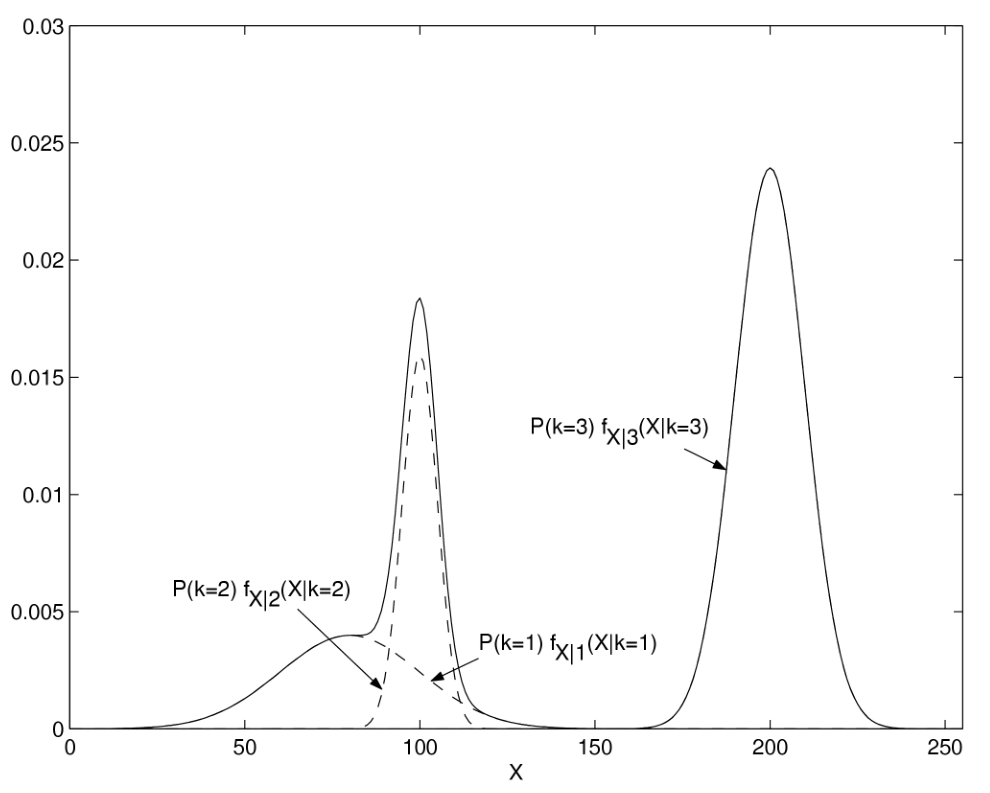
\includegraphics[width=\linewidth]{images/gaussian-mixture-model.png}
    \caption[Gaussian mixture model]{Gaussian mixture model\cite{power2002understanding}}
    \label{fig:gaussian-mixture-model}
\end{figure}

In order to apply the model to background subtraction problem, first step is to determine which of the $K$ states is most likely to give rise to current pixel values $\mathbf{X}=X$. The posterior probability $P(k|X,\Phi)$ is the likelihood that pixel value $X$ was generated by surface $k$. Using the Bayes's theorem:

$$ P(k|X,\Phi) = \frac{P(k)f_{\mathbf{X}|k}(X|k,\Phi)}{f_\mathbf{X}(X,\Phi)} $$
The k which maximizes the $P(k|X,\Phi) $ is considered to be the surface associated with $X$. Figure \ref{fig:gaussian-posterior-probability} illustrates the posterior probability $P(k|X,\Phi) $ as a function of $X$ for each $k\in \{  1,2,3 \}$ with the parameters in figure \ref{fig:gaussian-mixture-model}.

$$ \hat{k}=\operatorname*{argmax}_k P(k|X,\Phi)$$
\begin{figure}
    \centering
    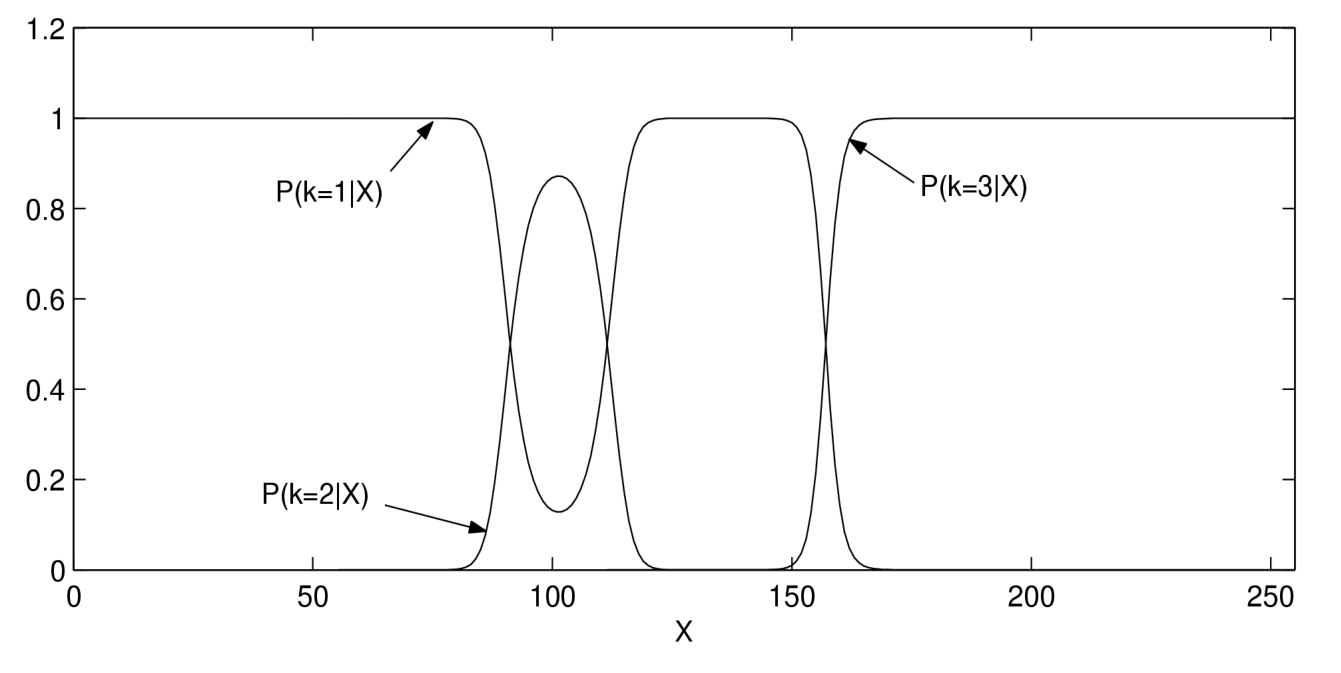
\includegraphics[width=\linewidth]{images/gaussian-posterior-probability.PNG}
    \caption[Posterior probability]{Posterior probability  $P(k|X,\Phi) $\cite{power2002understanding}}
    \label{fig:gaussian-posterior-probability}
\end{figure}


Once $X$ has been associated with a particular surface $\hat{k}$, it needs to be determined whether $\hat{k}$ is a foreground surface or background. 

The procedure for demarcation starts with ranking K states by $w_k / | \Sigma_k |$ in decreasing order. This ratio is proportional to height of weighted distribution $w_k f_{\mathbf{X}|k}(X|k,\theta_k)$. A surface $k$ is considered to be 
background if it occurs more frequently (higher $w_k$) and does not vary much (low $|\Sigma_k|$).  To separate the foreground and background surfaces, an overall prior probability $T$ of anything being in the background is used. The first $B$ of the ranked  states whose accumulated probability crosses the threshold $T$ are considered to be background. 
$$ B=\operatorname*{argmin}_b (\sum_{j=1}^b w_{j} > T)$$ 

\subsection{Stage 2 }
As mentioned before, goal of this stage is to verify human trespassing in case of activity. We implement this stage using Faster-RCNN\cite{ref_fasterrcnn}. Faster-RCNN is an object detection algorithm which takes in an image and predicts different objects in the image with their corresponding labels and bounding boxes. This is known as object detection and localization task which is different from the classification task (human trespassing/other activity) which we attemp to solve. We employ a simple an straight forward methodology to convert the Faster-RCNN output to our required output. If Faster-RCNN predicts at least one person with a probability greater than threshold $\tau$, then we label the input frame $f_i$ as showing trespassing activity. Otherwise we label it as a frame showing other activity. 

Faster-RCNN has three main components/sub-networks (figure \ref{fig:faster-rcnn-pipeline})
\begin{enumerate}
    \item Feature extraction (Conv Net)
    \item Region Proposal Net (RPN)
    \item Fast-RCNN head
\end{enumerate}

\subsubsection{Feature extraction}
This component/sub-network takes in the input image and produces convolution features. These convolutional features will be used by further sub-networks to predict the proposals and detections. This sub-network is also known as the backbone of network as it is responsible for producing high-quality, highly-discriminative features. This sub-stage is flexible in the sense that it can use any feature extraction network such as VGG or resnet. Recent implementations also employ FPN\cite{lin2017feature} to improve the discriminative power of this sub-stage. In our experiments, we used Resnet-50 with FPN. 

\begin{figure}
    \centering
    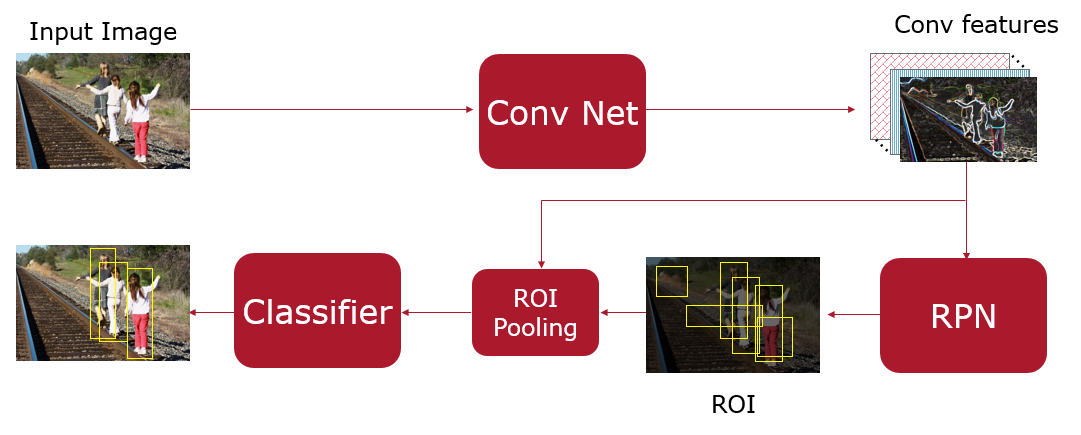
\includegraphics[width=\linewidth]{images/faster-rcnn-pipeline.PNG}
    \caption[Faster-RCNN pipeline]{Faster-RCNN pipeline}
    \label{fig:faster-rcnn-pipeline}
\end{figure}

\subsubsection{Region Proposal Network (RPN)}
\label{sec:RPN}
This sub-stage as the name suggests is responsible for proposing regions (rectangles) potentially containing objects. The idea of proposing regions using a neural network was proposed by Faster-RCNN for the first time. They also proposed the novel idea of anchors. As seen in figure \ref{fig:faster-rcnn-pipeline}, this sub-stage takes in the feature map and produces a list of proposals for the given image. Each proposal consists of binary label and proposed bounding box of the region of interest. The label indicates whether the proposal corresponds to an object or background. The proposals thus produced by the network are subjected to non-maximum suppression. This process removes the duplicate proposals and makes subsequent processing more efficient.  

\textbf{a) Anchor} \\
The novel idea of anchor has been introduced by Faster-RCNN. Anchor act as default region proposals. Their idea has been motivated from multi-scale sliding windows. Suppose we use a feature extraction convolutional network such that it converts a $800\times800$ image to $50\times50$ feature map (figure \ref{fig:anchors}). This means every $(x,y)$ location on feature map corresponds to $16\times16$ patch/window on original image. Similarly, $8\times8$ window on feature map corresponds to $128\times128$ window on original image. This $8\times8$ window on feature map is known as anchor. Faster-RCNN proposes multi-scale, multi-aspect ratio anchors. A total of 3 scales (8, 16, 32 on feature map) with 3 aspect ratios ($1:1$, $1:2$, $2:1$) produces 9 anchors on each $(x,y)$ location on feature map. Since, we have $50\times50$ locations, therefore this setting produces 22,500 anchors in total. However, in practice we use less than that. All the anchors whose regions lie outside feature map (eg. anchors near edges); they don't participate in training the network. 

\begin{figure}
    \centering
    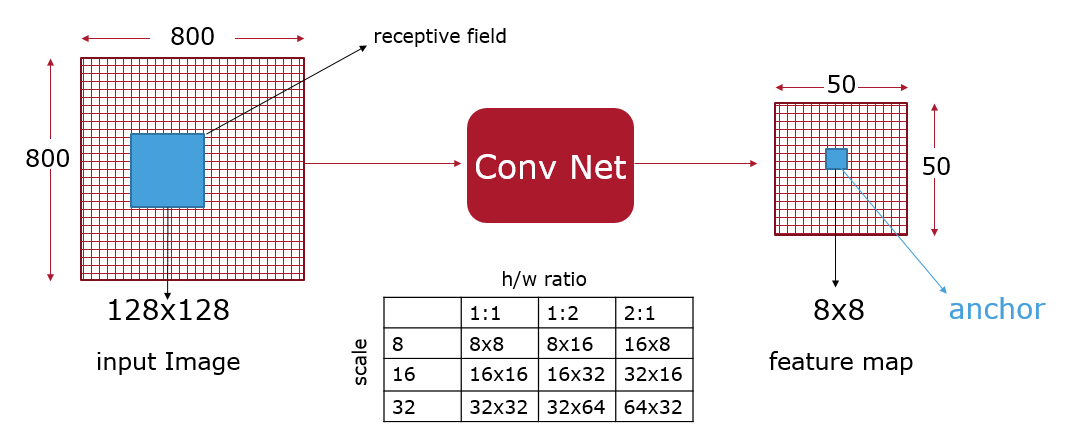
\includegraphics[width=\linewidth]{images/anchors.PNG}
    \caption[Anchor illustration]{Anchor illustration}
    \label{fig:anchors}
\end{figure}

\textbf{b) Architecture} \\
Figure \ref{fig:RPN-architecture} shows the architecture of RPN sub-network. Input to this network is the features generated by backbone network. These features are passed through a $3\times3$ ``same\footnote{$(h,w)$ of input and output feature map remains same by automatic padding}'' convolution layer. Faster-RCNN uses 515 output feature depth for this layer. Output of this layer is fed to the bounding box regressor layer and objectness layer which predicts bounding box locations and objectness score simultaneously. Both of these layers are modeled with $1\times1$ convolution. Bounding box regressor layer has $4k$ output depth where $k$ is the no. of anchors and 4 follows from the fact that each proposal is defined by 4 scalar values. For similar reasons, objectness layer has $2k$ output features. Thus each anchor produces a proposal. All of these proposals are post-processed by Non Maximum Suppression (NMS) discussed later. 

\begin{figure}
    \centering
    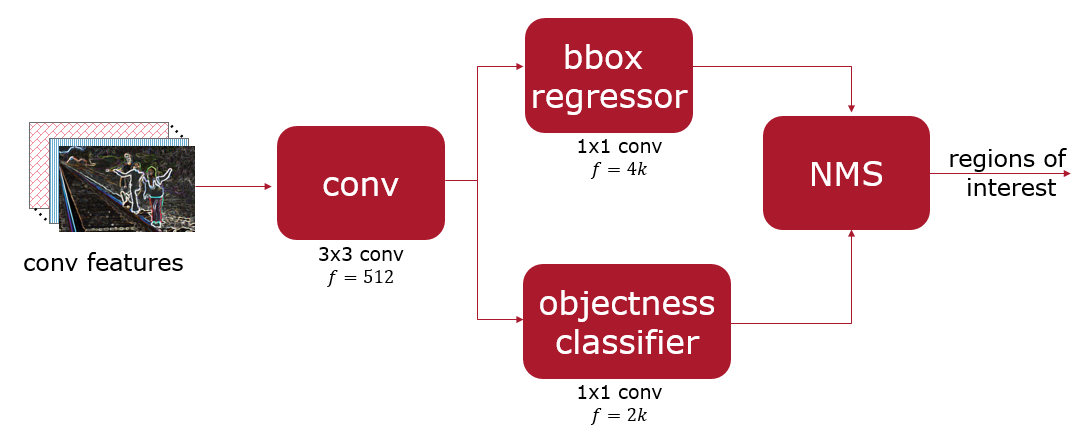
\includegraphics[width=\linewidth]{images/RPN-architecture.PNG}
    \caption[RPN architecture]{Region Proposal Network architecture}
    \label{fig:RPN-architecture}
\end{figure}

\textbf{c) Anchor targets} \\
While discussing the RPN architecture, we maintained that each anchor produces a proposal. Since, we shall train this network in a supervised manner therefore, we need targets corresponding to anchors. We shall use ground truth annotations to generate targets. Following steps need to be taken for anchor target generation.
\begin{enumerate}
    \item compute IoU for each anchor-target pair
    \item determine positive(negative) anchors and label them 
    \item confirm each ground truth is mapped to  at least on anchor 
\end{enumerate}

Step 1 is simple. Given an anchor $A_i$ and target bounding box $T_j$, we can compute Intersection over Union ($IoU(A_i,T_j)$) between them. Intersection over union is simply the ratio between area of overlap to area of union of two rectangles. Figure \ref{fig:iou} illustrates the concept of IoU graphically. Once we have IoU for each anchor-target pair, we can proceed to step 2. For each anchor $A_i$, it is matched to ground truth bounding box $T_{\hat{j}}$ such that $A_i$ has maximum IoU with $T_{\hat{j}}$ over all ground truth bounding boxes. In other words

$$ \hat{j} = \operatorname*{argmax}_{j} \{ IoU(A_i,T_j) \} $$

If $IoU(A_i,T_{\hat{j}}) > 0.7$, then $A_i$ is assigned positive label i.e. this this anchor corresponds to an object and $A_i$ will regress to bounding box of $T_j$. If $IoU(A_i,T_{\hat{j}}) < 0.3$, then $A_i$ is assigned negative label i.e. anchor corresponds to background. However, background anchors do not contribute towards bounding box regression learning process. 

\begin{figure}
    \centering
    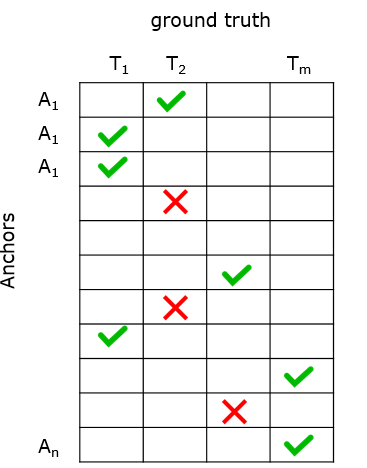
\includegraphics[width=0.5\linewidth]{images/anchor-targets.PNG}
    \caption[Anchor target assignment]{Anchor target assignment. Green tick indicates anchor assignment to ground truth object and red cross indicates background anchor assignment.}
    \label{fig:anchor-targets}
\end{figure}


\begin{figure}
    \centering
    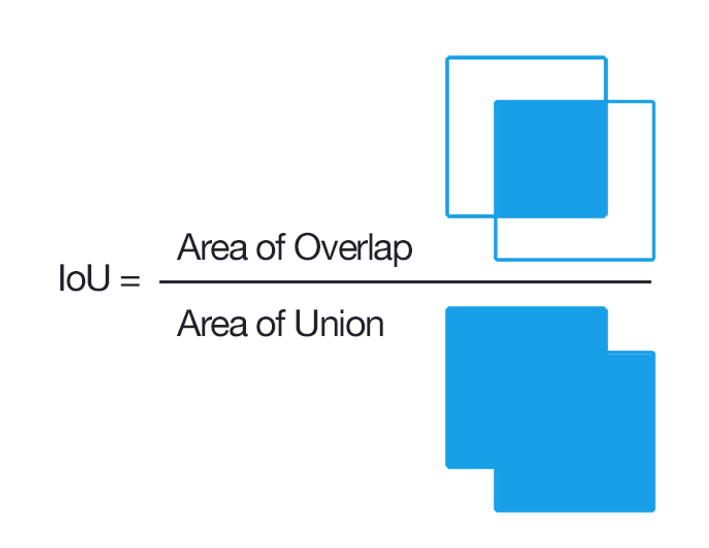
\includegraphics[width=0.5\linewidth]{images/iou.PNG}
    \caption{Intersection over Union}
    \label{fig:iou}
\end{figure}


\textbf{d) Non Maximum Suppression (NMS)} \\
As indicated in section \ref{sec:RPN}, NMS is responsible for removing the duplicate predictions. Figure \ref{fig:nms} illustrates the goal of this process graphically. In order to suppress duplicate proposal predictions with the less confidence, first step is to sort all the proposals in descending order. The first proposal is made  the reference proposal and pushed to ``keep'' list. IoU of this reference proposal with all the remaining proposals is computed and the proposals which sufficiently overlap with the reference proposal (IoU > 0.7) are discarded. They are considered to be the duplicate of reference proposal. In the next iteration the first proposal in the list of undecided proposals is made reference proposal and the process of first iteration is repeated. Again this leads to removal of all the proposals considered to be duplicate of reference proposal. The process continues on until all the proposals are decided i.e. either kept or discarded. Output of this process is the list of kept proposals. 


\begin{figure}
    \centering
    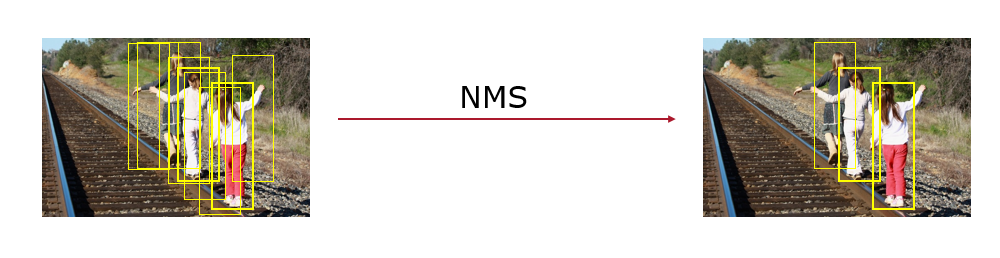
\includegraphics[width=\linewidth]{images/nms.PNG}
    \caption[Non Maximum Suppression (NMS)]{Non Maximum Suppression (NMS). Highly overlapping predictions with lesser confidence are suppressed.}
    \label{fig:nms}
\end{figure}

\subsubsection{Fast-RCNN head}
Once we have the proposals from RPN, we need to predict the corresponding objects' labels and location. This is done by Fast-RCNN head. Fast-RCNN consists of two components: 1) convolutional feature extraction and  2) head. Since, we have already computed the features, we only need the Fast-RCNN head to do the remaining task. Fast-RCNN head itself has two further sub-components. First one is Region of Interest (RoI) pooling and second one is classifier layer. Input to the Fast-RCNN head will be proposal feature maps and output shall be improved bounding box locations of corresponding proposals along with class labels. 


\textbf{a) Region of Interest (RoI) Pooling} \\
Different proposals have different feature map sizes. However, the classifier expects them to be of same size. This process (RoI pooling) is responsible for converting variable sized feature maps into fixed sized. The methodology used by Fast-RCNN in this case is quite simple. Suppose a feature map of size $n\times m$ has to be converted to $a \times b$ size. Then, a grid of size $a \times b$ is placed on top of feature map and maximum feature value from each grid cell is copied to corresponding cell in output buffer. this converts a $n\times m$ feature map to a size of $a \times b$. Figure \ref{fig:roi-pooling} illustrates the concept by an example. In this case, feature map of size $5 \times 7$ is converted to $2 \times 2$.

\begin{figure}
    \centering
    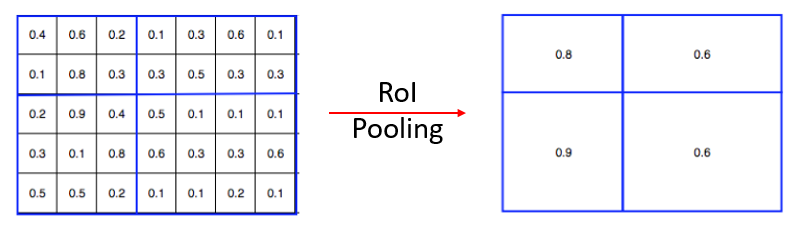
\includegraphics[width=\linewidth]{images/roi-pooling.PNG}
    \caption{RoI pooling}
    \label{fig:roi-pooling}
\end{figure}

\textbf{b) Classifier} \\
Once RoI pooling has adjusted the size of feature map to fixed dimensions, the feature maps are ready to be fed to classifier. The classifier takes in those features and pass them through two fully connected layers. The output of those two layers is fed to two separate fully connected layers responsible for predicting bounding boxes and object class labels. The bounding boxes and labels so predicted are the final output of Faster-RCNN. Figure \ref{fig:classifier} illustrates the architecture of classifier.

\begin{figure}
    \centering
    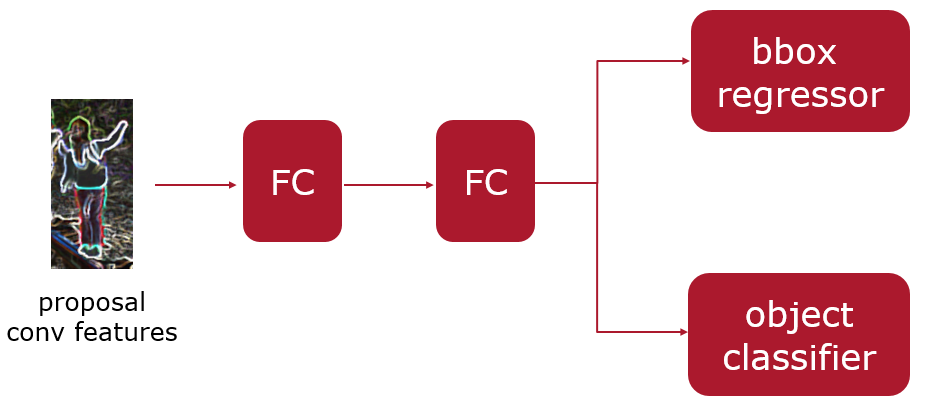
\includegraphics[width=\linewidth]{images/classifier.PNG}
    \caption{Fast-RCNN classifier}
    \label{fig:classifier}
\end{figure}


\subsubsection{Training loss}
While training the Faster-RCNN, we train two sub-networks: RPN and classifier. Both of these networks have two objectives: label classification and bounding box regression. Following two equations indicate the RPN and classifier loss. First term corresponds to label classification and second term corresponds to bounding box regression. 

$$Loss_{RPN}= \frac{1}{N_{cls}}\sum_i L_{cls}(\hat{p}_i,p_i) + \frac{\lambda_r}{N_{reg}}\sum_i p_i L_{reg}(\hat{t}_i,t_i)$$
$$Loss_{classifier} = \frac{1}{N_{cls}}\sum_i L_{cls}(\hat{q}_i,q_i) + \frac{\lambda_c}{N_{reg}}\sum_i [q_i > 0] L_{reg}(\hat{u}_i,u_i)$$

where \\
$\hat{p}_i=$ anchor label prediction \\
$\hat{t}_i=$ anchor bounding box prediction \\
$\hat{q}_i=$ RoI label prediction \\
$\hat{u}_i=$ RoI bounding box prediction \\
${p}_i=$ anchor ground truth label \\
${t}_i=$ anchor bounding box  \\
${q}_i=$ RoI ground truth label  \\
${u}_i=$ RoI ground truth bounding box  \\
$\lambda_r =$ RPN loss balance coef. \\
$\lambda_c =$ classifier loss balance coef. \\
$N_{cls}=$ mini-batch size \\
$N_{reg}=$ total anchors

Classification loss $L_{cls}$ is the standard log loss and regression loss $L_{reg}$ is the smooth-$L_1$ loss as defined below. 

$$ L_{cls}(\hat{y},y) = -\sum_j y_jlog(\hat{y}_j) $$
$$ L_{reg}(\hat{b},b) = \sum_{j=1}^4 SL_1(\hat{b}_j - b_j) $$
$$SL_1(x) = \begin{cases}
0.5x^2, & \text{if } |x|<1 \\
x-0.5,  & \text{otherwise}
\end{cases}
$$
where input parameters to each function carry standard meaning. 

Total loss of the network is simply the sum of RPN loss and classifier loss.
$$ Loss = Loss_{RPN} + Loss_{classifier} $$

Apart from that notice the term $p_i$ in regression term of RPN loss. This makes sure that regression loss is activated only if proposal corresponds to an object, not the background.  Thus bounding box predictions corresponding to background proposals do not contribute towards training. Furthermore, the expression $[q_i>0]$ does a similar job in classifier loss. This again acts as a flag to add regression loss only corresponding to actual objects and not the background. 

$\lambda_r$ and $\lambda_c$ act as the balancing parameter  between label classification and bounding box regression. The authors of Faster-RCNN claim that $\lambda_r$ is redundant and Faster-RCNN remains insensitive to a large range of $\lambda_r$. 



\newpage














